\section{Background on Coupled Architectures} \label{sec:background}
Modern CPU has evolved into powerful processor with multi-core and high frequency processing capabilities. However, due to the manufacturing limitations and thermal issues, it becomes increasingly difficulty to further improve the computing capability of CPU. Moreover, the increasing complex applications require processors to be able to process workloads with varying computing complexity and pattern. Accelerators are designed to bridge the gap between CPU and requirements in reality. Graphics Processing Unit (GPU) is specifically designed for manipulating graphic and image processing. Field Programmable Gate Array (FPGA) is specialized with configurable capability to deliver combinational functions customized by users.

\subsection{Why coupled}
Since the emerging of accelerators, they are designed to serve specific purposes. In a long time, heterogeneous systems equipped with CPU and dedicated accelerators have been widely adopted in various domains. On the one hand, heterogeneous systems can be provide additional computing capability beyond CPU-based systems. On the other hand, accelerators in such systems can process the parts of complex workloads with specialized requirements faster than CPU. As video stream processing involves large amount of computations and the video stream usually has a limited lifetime, resulting that it is not well suited to CPU as caches cannot be fully utilized. On the contrary, accelerators like GPU work efficiently on such workloads as it has greatly simplified memory hierarchy and control logics. Instead, more hardware resources are devoted to light-weight and massively parallel Arithmetic Logic Units (ALUs) that is suitable for such workloads. More generally, transistors in CPU are dedicated to branch prediction, out of order logic and caching to reduce the latency to memory, thus the performance of each thread is maximized. However, most transistors of GPU are concentrated on ALUs and registers, thus each thread's state can be stored, allowing faster context switching between threads to cover, rather than to reduce, the latency to memory.

Though integrating accelerators into the system has eased the burden of CPU to process complex workloads much faster and more efficiently, additional overhead is incurred, hindering its wider adoption to obtain further performance improvements.

Firstly, most traditional systems incorporate CPU and accelerators connected via PCI-e to transfer data between them. Though each processor has enough hardware space so that they can be designed powerful enough, the data transfer overhead and coordination between CPU and accelerators make it inefficient to run applications on the system. On the one hand, the bandwidth of PCI-e is limited (e.g., 4~8 GB/sec). On the other hand, the performance of PCI-e seriously downgrades in cases where the size of data blocks is small.

Secondly, due to the data transfer overhead, workloads are usually offloaded to accelerators for processing as a whole. Once computations end, the entire results are transferred back to the CPU for post-processing. Such naive workload scheduling is PCi-e favoured. However, it always results in imbalance between CPU and accelerators. The CPU is always idle while the accelerator is busy with compute-intensive workloads.

Thirdly, traditional applications on CPU+accelerator platforms do not consider the dynamics in complex applications due to hardware constraints. Complex applications always involve various kernels with narrow and wide vectors, or different stages may involve varying degree of parallelism so that the hardware configuration should be adapted accordingly online to satisfy the varying requirements. As the traditional hardware is absent from capabilities like nested or dynamic parallelism, programmers have to carefully design and tune their programs to avoid hardware resource underutilization.

Fourthly, as the frequency and the number of transistors significantly increase in CPU and accelerators, the heat dissipation and power requirements increase as well. It becomes unacceptable in in modern scientific applications that are usually deployed on large scale clusters equipped with hundreds or even thousands of nodes. Power consumption should be reviewed in modern times as environment-friendly is one of most important issues for sustainable earth.

Fifthly, as accelerators are originally designed for specific purposes, coding for them has always posed a special challenge for software developers due to great differences in hardware architectures across accelerator vendors, or even across generations of accelerations from the same vendor. For example, programming on GPU requires knowledge about image rendering and the GPU hardware specifics. The programming languages such OpenGL or GLSL requires users to abstract the general-purpose applications to fit for GPU rendering model. Besides, all these accelerators have their own Instruction Set Architecture (ISA) that is different from CPU's ISA (like x86). Therefore, communication between CPU and accelerators can be only achieved by dedicatedly designed interfaces and controlled by users. This inevitably imposes additional overhead to users. Optimal performance cannot be guaranteed.

To address the above issues, vendors have revisited the traditional architectural design and released an innovative architecture, where accelerators (like GPU and FPGA) are more tightly coupled with CPU in the same die, eliminating the PCI-e bus by incorporating much faster data paths. Moreover, some new features are introduced to enable software developers with more programming flexibility to deploy applications on such coupled architectures to exploit the great computing power while avoiding the long standing performance bottlenecks.

\subsection{Existing products}
As a promising architectural design trend, hardware vendors have released various coupled architectures to satisfy different requirements.

Since the release of Nvidia G80, GPU has become a popular accelerator to speed up applications with intensive computations and high parallelism on large amount of data. With the increasing adoption of coupled architectures, coupled CPU-GPU architectures demonstrate the advantages over the discrete platforms. In 2011, AMD released its first generation Accelerated Processing Units (formerly known as \textit{Fusion}). In Fusion, the CPU and the GPU are integrated in the same chip, sharing the memory subsystem including main memory and Last Level Cache (LLC). Intel released its early stage products Sandy Bridge (in 2011) and Ivy Bridge (in 2012). In these products, CPU and integrated GPU are collected with ring bus which is collected to the main memory and LLC, so that data sharing between the CPU and the GPU becomes more efficient. Later, in its Iris series products, embedded Dynamic Random-Access Memory (eDRAM) is introduced into system to work as a L4 cache with much larger size (128MB) to share data between the CPU and the GPU. Nvidia also proposed a \textit{Denver Project} with intention to integrate its ARM-based CPU with a broad range of accelerators such as GPU and Digital Signal Processor (DSP).

\jiong{Here maybe Zeke could help to verify as he is familiar with FPGA.} FPGA is an integrated circuit designed to be configured by customers after manufacturing, making it possible to be adapted according to the dynamics to achieve the optimal processing performance on each specific algorithm. Usually it is connected to the CPU via PCI-e bus. In 2016, Intel has launched a processor which integrates Broadwll Xeon with Altera Arria 10 FPGA. Quick Path Interconnect (QPI) is used to connect these hardware components for fast and efficient communication.

\jiong{Should there be a table? What contents?}

\subsection{Abstract Coupled Architectures}
Heterogeneous architectural designs are emerging in the field of computer architecture. Researchers have been proposing different heterogeneous designs in the modern/future processors, which attempt to improve the performance, reduce the energy consumption or both. Among these designs, coupled architectures are becoming increasingly important across a large amount of applications running on platforms ranging from servers to embedded devices.

Though there are some differences in the techniques used by vendors to implement their own coupled architectures, their general design methodologies are similar with each other. We illustrate the abstracted coupled architecture design in Figure \ref{fig:generalcoupledsystem}. As shown in Figure \ref{fig:generalcoupledsystem}, CPU and accelerator are connected with specialized interconnection techniques (such as QPI, ring bus or unified north bridge). In such way, data transfers are more efficient and flexible than ever before, enabling users put more efforts on the logic design. The memory system including cache and main memory is also shared between CPU and accelerator. With various coherence reserving policies, the shared cache can be used as a working sharing hub between two sides with appropriate algorithmic design.
\begin{figure}
	\centering
    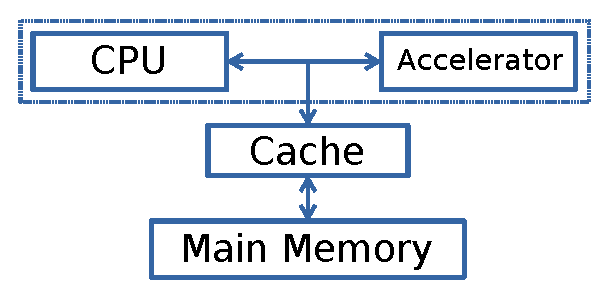
\includegraphics[width=0.45\textwidth]{figures/generalCoupledSystem.eps}
    \caption{Abstract coupled architectures.} \label{fig:generalcoupledsystem}
\end{figure}

To ease software developers from error-prone coding on cross platforms, a unified programming langauge, Open Computing Language (OpenCL), originally proposed by Apple Inc. becomes the standard programming language on heterogeneous platforms consisting of CPUs, GPUs, DSPs, FPGAs and other processors or hardware acceleratros. OpenCL programs can be coded once and run on any OpenCL-compatible devices. Existing studies \cite{Fang2011, Thouti2012} have shown that programs in OpenCL can achieve very close performance to those in platform-specific languages such as CUDA for NVIDIA GPUs and OpenMP for CPUs. For example, Fang et al. [11] demonstrate that the CUDA-based implementations are at most 30\% better than OpenCL-based implementations on NVIDIA GPUs. On CPUs, OpenCL even outperforms OpenMP in many applications \cite{Thouti2012}.

All OpenCL-compatible devices are mapped to the same logical architecture as shown in Figure \ref{fig:gpuarchitecture}, namely compute device. Each compute device consists of a number of Compute Units (CUs). Furthermore, each CU contains multiple processing elements running in the SPMD style. As the CPU is also OpenCL-compatible, systems consisting of CPU and other OpenCL-compatible accelerators are treated as two coupled OpenCL devices. The code piece executed by a specific device is called a kernel. A kernel employs multiple work groups for the execution, and each work group contains a number of work items. A work group is mapped to a CU, and multiple work items are executed concurrently on the CU. The execution of a work group on the target architecture is vendor-specific. For instance, AMD usually executes 64 work items in a wavefront and NVIDIA with 32 work items in a warp. All the work items in the same wavefront run in the Single Instruction Multiple Data (SIMD) manner. On FPGA, each OpenCL kernel is compiled to a custom circuit. The operations within the kernel are implemented using the ALMs and DSPs, forming sub-circuits that are wired together according to the data flow of the algorithm. Load/store units allow access to different memory areas.

\begin{figure}
	\centering
    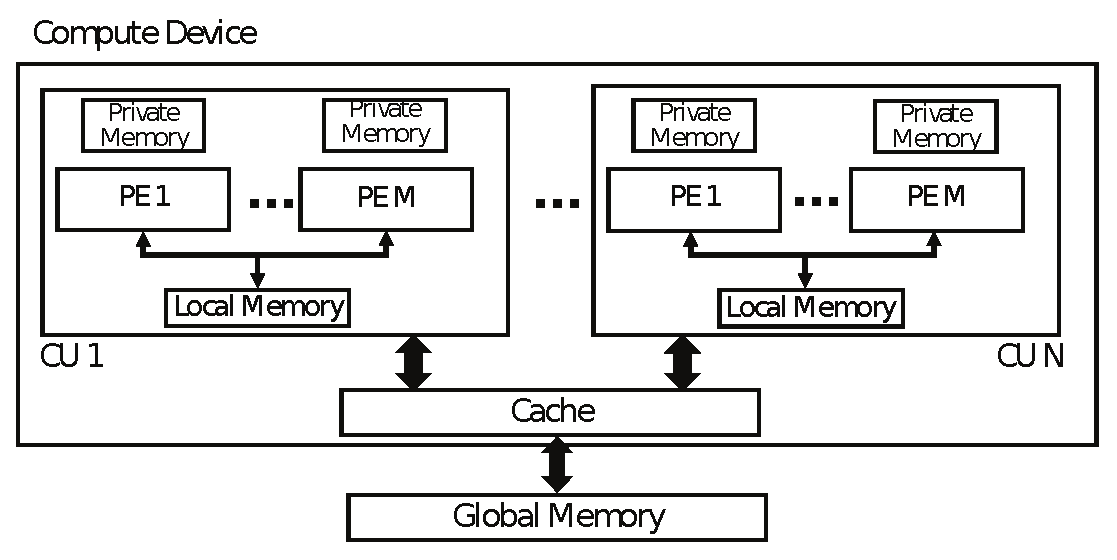
\includegraphics[width=0.90\textwidth]{figures/gpuarchitecture.eps}
    \caption{Hardware abstraction in OpenCL.} \label{fig:gpuarchitecture}
\end{figure}

